% Options for packages loaded elsewhere
\PassOptionsToPackage{unicode}{hyperref}
\PassOptionsToPackage{hyphens}{url}
\PassOptionsToPackage{dvipsnames,svgnames,x11names}{xcolor}
%
\documentclass[
]{jds}

\usepackage{amsmath,amssymb}
\usepackage{iftex}
\ifPDFTeX
  \usepackage[T1]{fontenc}
  \usepackage[utf8]{inputenc}
  \usepackage{textcomp} % provide euro and other symbols
\else % if luatex or xetex
  \usepackage{unicode-math}
  \defaultfontfeatures{Scale=MatchLowercase}
  \defaultfontfeatures[\rmfamily]{Ligatures=TeX,Scale=1}
\fi
\usepackage{lmodern}
\ifPDFTeX\else  
    % xetex/luatex font selection
\fi
% Use upquote if available, for straight quotes in verbatim environments
\IfFileExists{upquote.sty}{\usepackage{upquote}}{}
\IfFileExists{microtype.sty}{% use microtype if available
  \usepackage[]{microtype}
  \UseMicrotypeSet[protrusion]{basicmath} % disable protrusion for tt fonts
}{}
\makeatletter
\@ifundefined{KOMAClassName}{% if non-KOMA class
  \IfFileExists{parskip.sty}{%
    \usepackage{parskip}
  }{% else
    \setlength{\parindent}{0pt}
    \setlength{\parskip}{6pt plus 2pt minus 1pt}}
}{% if KOMA class
  \KOMAoptions{parskip=half}}
\makeatother
\usepackage{xcolor}
\setlength{\emergencystretch}{3em} % prevent overfull lines
\setcounter{secnumdepth}{-\maxdimen} % remove section numbering
% Make \paragraph and \subparagraph free-standing
\makeatletter
\ifx\paragraph\undefined\else
  \let\oldparagraph\paragraph
  \renewcommand{\paragraph}{
    \@ifstar
      \xxxParagraphStar
      \xxxParagraphNoStar
  }
  \newcommand{\xxxParagraphStar}[1]{\oldparagraph*{#1}\mbox{}}
  \newcommand{\xxxParagraphNoStar}[1]{\oldparagraph{#1}\mbox{}}
\fi
\ifx\subparagraph\undefined\else
  \let\oldsubparagraph\subparagraph
  \renewcommand{\subparagraph}{
    \@ifstar
      \xxxSubParagraphStar
      \xxxSubParagraphNoStar
  }
  \newcommand{\xxxSubParagraphStar}[1]{\oldsubparagraph*{#1}\mbox{}}
  \newcommand{\xxxSubParagraphNoStar}[1]{\oldsubparagraph{#1}\mbox{}}
\fi
\makeatother


\providecommand{\tightlist}{%
  \setlength{\itemsep}{0pt}\setlength{\parskip}{0pt}}\usepackage{longtable,booktabs,array}
\usepackage{calc} % for calculating minipage widths
% Correct order of tables after \paragraph or \subparagraph
\usepackage{etoolbox}
\makeatletter
\patchcmd\longtable{\par}{\if@noskipsec\mbox{}\fi\par}{}{}
\makeatother
% Allow footnotes in longtable head/foot
\IfFileExists{footnotehyper.sty}{\usepackage{footnotehyper}}{\usepackage{footnote}}
\makesavenoteenv{longtable}
\usepackage{graphicx}
\makeatletter
\def\maxwidth{\ifdim\Gin@nat@width>\linewidth\linewidth\else\Gin@nat@width\fi}
\def\maxheight{\ifdim\Gin@nat@height>\textheight\textheight\else\Gin@nat@height\fi}
\makeatother
% Scale images if necessary, so that they will not overflow the page
% margins by default, and it is still possible to overwrite the defaults
% using explicit options in \includegraphics[width, height, ...]{}
\setkeys{Gin}{width=\maxwidth,height=\maxheight,keepaspectratio}
% Set default figure placement to htbp
\makeatletter
\def\fps@figure{htbp}
\makeatother

\makeatletter
\@ifpackageloaded{caption}{}{\usepackage{caption}}
\AtBeginDocument{%
\ifdefined\contentsname
  \renewcommand*\contentsname{Table of contents}
\else
  \newcommand\contentsname{Table of contents}
\fi
\ifdefined\listfigurename
  \renewcommand*\listfigurename{List of Figures}
\else
  \newcommand\listfigurename{List of Figures}
\fi
\ifdefined\listtablename
  \renewcommand*\listtablename{List of Tables}
\else
  \newcommand\listtablename{List of Tables}
\fi
\ifdefined\figurename
  \renewcommand*\figurename{Figure}
\else
  \newcommand\figurename{Figure}
\fi
\ifdefined\tablename
  \renewcommand*\tablename{Table}
\else
  \newcommand\tablename{Table}
\fi
}
\@ifpackageloaded{float}{}{\usepackage{float}}
\floatstyle{ruled}
\@ifundefined{c@chapter}{\newfloat{codelisting}{h}{lop}}{\newfloat{codelisting}{h}{lop}[chapter]}
\floatname{codelisting}{Listing}
\newcommand*\listoflistings{\listof{codelisting}{List of Listings}}
\makeatother
\makeatletter
\makeatother
\makeatletter
\@ifpackageloaded{caption}{}{\usepackage{caption}}
\@ifpackageloaded{subcaption}{}{\usepackage{subcaption}}
\makeatother

\ifLuaTeX
  \usepackage{selnolig}  % disable illegal ligatures
\fi
\usepackage[]{natbib}
\bibliographystyle{plainnat}
\usepackage{bookmark}

\IfFileExists{xurl.sty}{\usepackage{xurl}}{} % add URL line breaks if available
\urlstyle{same} % disable monospaced font for URLs
\hypersetup{
  pdftitle={My wonderful paper},
  colorlinks=true,
  linkcolor={blue},
  filecolor={Maroon},
  citecolor={Blue},
  urlcolor={Blue},
  pdfcreator={LaTeX via pandoc}}


\title{My wonderful paper}
\author{}
\date{}

\begin{document}
\maketitle
\begin{abstract}
Unexpected results in data analysis can prompt researchers to examine
data quality and analysis steps. While some researchers can typically
diagnose issues effectively with a few checks, others may struggle to
identify appropriate checks to diagnose the problem. {[}an example of
check{]} These checks are often informal and difficult to trace and
discuss in publications, resulting in others questioning the
trustworthiness of the analysis. To address this, we formalize the
informal checks into an \emph{analysis plan} that encompasses the
analysis steps and (the unit tests): one test for whether the result
meets expectations and multiple tests for checking the analysis. We then
present a procedure to assess the quality of these unit tests based on
their accuracy and redundancy on simulated versions of the original
data. The accuracy is assessed using binary classification metrics,
\emph{i.e.}, precision and recall, while redundancy is calculated using
mutual information. This procedure can be used to conduct a sensitivity
analysis, compare different analysis plans, and to identify the optimal
cutoff point for the unit tests.
\end{abstract}

\renewcommand*\contentsname{Table of contents}
{
\hypersetup{linkcolor=}
\setcounter{tocdepth}{3}
\tableofcontents
}

\newpage

\section{Introduction}\label{introduction}

\begin{itemize}
\tightlist
\item
  emphasize trustworthy data science since it is the theme of the
  special issue
\end{itemize}

In a data analysis, an experienced researcher can often quickly assess
whether a result meets their expectation, while others may be unsure of
what to anticipate from the analysis or how to recognize when results
diverge form expected norms. (These expectations are often based on
prior knowledge, domain expertise, or common sense and they can often be
framed into a Boolean question that can be answered by a unit test. For
example, in a linear regression model, one may expect the p-value of the
coefficient to be less than 0.05. On top of the expectation on the final
results, researchers may also have expectations on the intermediate
steps of the analysis process. For example, one may expect the data
doesn't contain outliers, etc. These expectations are often checked
early on to prevent an unexpected propagate through the analysis
process.)

This expectation-setting process is often implicit and rarely documented
or discussed in publications. (There are most publication requires open
source code for publication, however, it is no instruction or guidance
on checking \ldots). Yet, making them explicit is crucial for 1) helping
junior researchers interpret results and diagnose the unexpected, 2)
providing checkpoints that support independent replication or
application of methods to new data, 3) aligning assumption across
researchers from different backgrounds.

In this paper, we formalize these informal checks into an \emph{analysis
plan} comprising the analysis steps along with the associated unit
tests. This formalization allows us to examine assumptions made about
the data during analysis and to compare different unit tests in
diagnosing unexpected outcomes. We then introduce a procedure to assess
the quality of these unit tests based on their accuracy and redundancy
across simulated version of the original data. The accuracy is assessed
using binary classification metrics -- precision and recall -- while
redundancy is measured using mutual information. The workflow provides
numerical guarantee of the consistency of the expectation and the data
for the analysis plan. This means that given the assumption of the data
generating mechanism, the analysis will provide the outcome we expect.
In data analysis, analysts are not necessarily collecting the data and
they can only make reasonable assumption about the quality of the data.
This method we propose provides a numerical guarantee, based on
simulation, that the analysis will produce the outcome we expect, given
the assumption of the data generating mechanism. This provides
transparency of the analysis and build trustworthy data analysis.

The rest of the paper is organized as follows: Section~\ref{sec-plan}
describes the concept of analysis plan in detail.
Section~\ref{sec-examples} provides examples of analysis plan {[}more
details{]}. (need another section here or before examples?)
Section~\ref{sec-conclusion} concludes the paper.

\section{Literature review}\label{literature-review}

\subsection{Diagnosing unexpected outcomes in data
analysis}\label{diagnosing-unexpected-outcomes-in-data-analysis}

\citep{peng_diagnosing_2021} describes three pedagogical exercises of
introducing diagnosing unexpected outcome into a classroom setting.

TODO: what if the expectation is ``wrong''

\subsection{Data analysis checks in statistical
software}\label{data-analysis-checks-in-statistical-software}

Currently, little has been done on how to computationally incorporate
this diagnostic approach into data analysis workflow or software. Most
of the diagnostic tools focus on defining user-specified rules, such as
data quality checks or producing metrics to summarize model performance,
as in model diagnostics. For example, the \texttt{assertr} package
\citep{assertr} and the \texttt{pointblank} package \citep{pointblank}
provide data validation tools to allow users to define data quality
checks. In contrast, packages provide model checks tools like
\texttt{performance} \citep{performance} and \texttt{yardstick}
\citep{yardstick}, from the \texttt{tidymodels} \citep{tidymodels}
ecosystem, offers goodness-of-fit, residual analysis, and model
performance metrics.

These packages provide the tools to conduct diagnostics but still don't
reflect the mental process of how data analysts diagnose the unexpected
output. For example, when an unexpected output occurs, an analyst may
check on whether a column in the data frame is between two values for
data quality. However, it is not documented what motivates the analyst
to conduct this check -- whether it also applies to other researchers
analyzing new data in the same contexts, whether it is a common practice
in the field, or whether it is a reaction to this particular data or
scenario. Currently, most of these assumptions are not discussed in the
publication or captured by tools themselves. While one might be able to
infer some of the mental process of the analysts from external sources,
such as talking to them or watching screencast videos produced by the
analysts e.g.~TidyTuesday screencast videos, these insights are not
systematically documented or made machine-readable. This gap highlights
the need for tools that provide higher level documentation of reasoning
behind the checks, facilitating a more transparent and interpretable
analysis process.

\subsection{Unit tests}\label{unit-tests}

Why develop unit tests in software engineering? Because it is difficult
to predict the outcome of a program, especially when the program is
complex. Because the loss associated with a program failure is costly.

Existing tools for checks in data analysis including those check for
data quality and model diagnostics. In software development,

\begin{itemize}
\tightlist
\item
  the \texttt{testthat} package \citep{testthat} provides the
  infrastructure for testing R code. It allows users to write unit tests
  for functions and packages.
\item
  The \texttt{assertthat} package \citep{assertthat} helps to write
  assertion statements that are supposed to be true at a certain point
  in the code for defensive programming.
\end{itemize}

\section{Analysis plan}\label{sec-plan}

\subsection{Framing checks into unit
tests}\label{framing-checks-into-unit-tests}

Q: Whether we should formulate these concept with math notation?? A:
only if it helps

An analysis plan is a set of analysis steps combined with expectations.
Expectations represent our belief about certain aspects of the analysis,
independent of the analysis itself. It can be divided into two types:
\emph{outcome expectation} and \emph{plan expectation}. Outcome
expectation refers to what we anticipate from the main result of the
analysis based on prior knowledge. They shape how we interpret the
results and assess whether they are consistent with existing knowledge
or indicate the need for updates \citep{grolemund_cognitive_2014}. For
example, in public health, prior research shows the average increase in
mortality rate per unit increase in PM10 is about 0.50\%
\citep{liu2019ambient}. This serves as an expectation for similar future
studies. Plan expectations concern the intermediate steps within the
analysis rather than the final outcome. They serve as checkpoints to
detect deflection in the analysis process For example, we may expect
temporal data to be ordered with no gaps and duplicates, or expect that
temperature will be a significant covariate in the linear regression
model of PM10 on mortality.

Experienced analysts often have implicit expectation about the outcome
and rely on a few ``directional signs'' to check when the outcome
deviate from those expectation. However, these expectations are rarely
made explicit within the analysis workflow. This makes it challenging
for consumers of the analysis to evaluate the results, since it becomes
difficult to disentangle whether discrepancies arise from differing
expectations or from the use of statistical technique, without running
the analysis themselves. Non-expert analysts, lacking prior knowledge or
instinct, may not have clear expectations of the results. This can lead
to reduced confidence of the analysis and makes it more difficult and
time-consuming to diagnose the cause of the deviation when the results
don't align with expectations. By explicitly formulating these
expectations, an analysis plan can guide the analysis process,
facilitate the communication and evaluate the validity of the results.

\subsection{A toy example}\label{a-toy-example}

Consider a 30-day step count goal. Suppose you resolve to walk at least
8,000 steps each day, using an app to record your daily step count. Your
target average is 9,000 steps per day, with some ``lows'' day, where you
walk around 4,000 steps and ``high'' days where you reach about 12,000
steps. After 30 days, you check how many times your step count fall
below 8,000 and aim for no more than five days under this threshold.

To simulation this data, three normal distributions with different means
are used for the daily step counts: \(\mathcal{N}(4000, 200)\) for low
days, \(\mathcal{N}(12000, 200)\) for high days, and
\(\mathcal{N}(9000, 300)\) for typical days. The number of low and high
days can be simulated from a Poisson distribution with \(\lambda = 4\).
Figure~\ref{fig-step-count} displays the number of days with fewer than
8,000 steps across 300 simulated 30-day periods.

In this scenario, the outcome expectation is that the number of days
with a step count below 8,000 will be no more than five. To diagnose
potential reasons why this outcome expectation might fail, we can
establish a few plan expectations. For example, if the average step
count is too low, this may suggest there are too many low days,
potentially lead to an unexpected outcome. Similarly, we can also check
the quantile of the step count, if more than a third of the days fall
below 8,000, this could indicate an excess of low-count days.
Additionally, we may may expect the standard deviation of the step count
not to be overly large.

These considerations yield the following three unit tests as plan
expectations:

\begin{itemize}
\tightlist
\item
  test1: the test fails if the mean step count is below 8,200
\item
  test2: the test fails if the 30th percentile of the step counts is
  below 8,200
\item
  test3: the test fails if the standard deviation of the step
  countsexceeds 2,500.
\end{itemize}

\phantomsection\label{cell-fig-step-count}
\begin{figure}[H]

\centering{

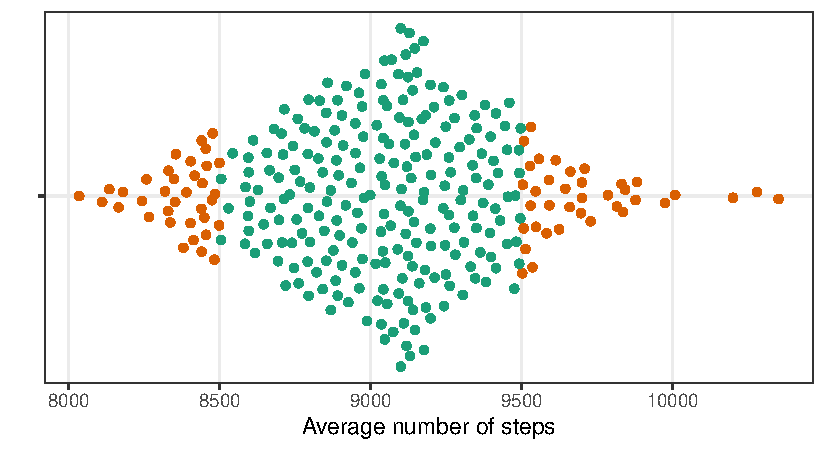
\includegraphics{index_files/figure-pdf/fig-step-count-1.pdf}

}

\caption{\label{fig-step-count}Number of days with fewer than 8,000
steps across 300 simulated 30-day periods. The orange bars indicate
instances where the count exeeds five days, representing an unexpected
outcome in this scenario.}

\end{figure}%

\textsubscript{Source:
\href{https://huizezhang-sherry.github.io/paper-analysis-plan/index.qmd.html}{Article
Notebook}}

\section{Method}\label{method}

\subsection{A workflow to assess the quality of unit
tests}\label{a-workflow-to-assess-the-quality-of-unit-tests}

In real-world applications, it is rare to create a set of unit tests can
fully guarantee expected results. On one hand, there is the cost of
effort involved in manually developing all these tests; on the other,
there is the inherent complexity of the problem. (can we - if we're
thriving for detecting 95\% of the cause?). However, the quality of unit
tests can be evaluated by simulated data. One set of tests is considered
better than another if a small set of tests can reliably detect
unexpected outcomes, which brings two criteria in the evaluation metric:
accuracy and parsimony. Figure~\ref{fig-metric-calc} illustrates the
workflow for calculating the metrics.

\phantomsection\label{cell-fig-metric-calc}
\begin{figure}[H]

\centering{

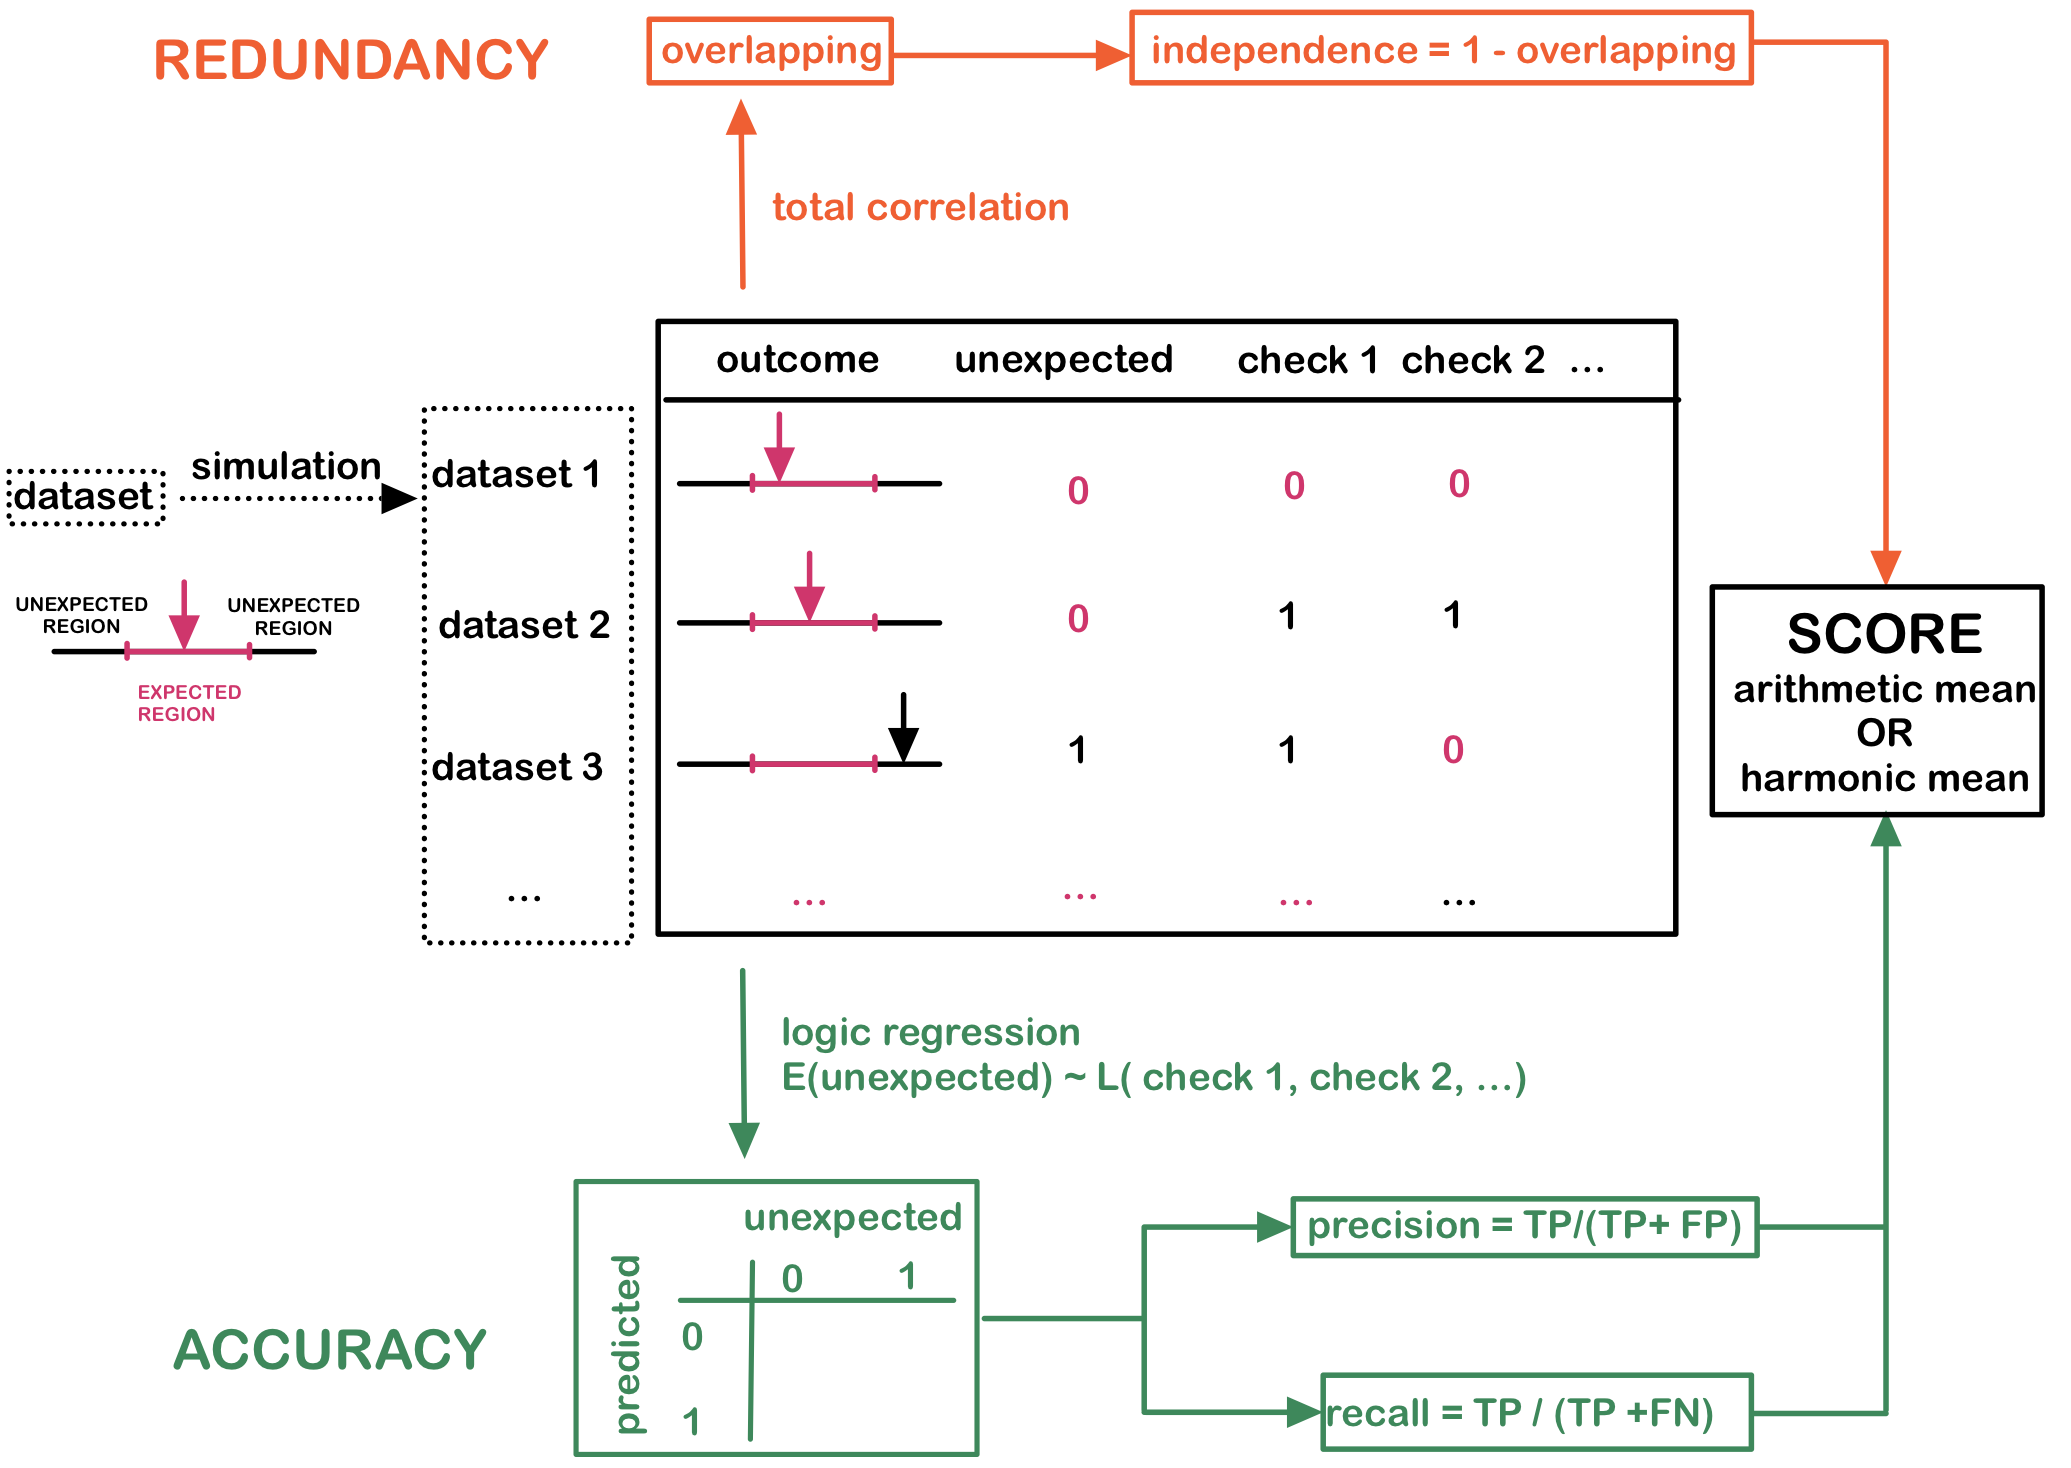
\includegraphics[width=6.73in,height=\textheight]{figures/metric-calc.png}

}

\caption{\label{fig-metric-calc}this is the cap}

\end{figure}%

\textsubscript{Source:
\href{https://huizezhang-sherry.github.io/paper-analysis-plan/index.qmd.html}{Article
Notebook}}

Accuracy refers to a set of tests' ability to accurately detect
unexpected outcomes while minimizing false positives and false
negatives. A false positive can indicate (caution or skepticism on
checking the data), whereas a false negative suggests the tests may lack
sensitivity to unexpected outcomes. To model the relationship between
the plan and outcome expectation (binary-binary), a logic regression
model is used \citep{ruczinski_logic_2003}. Originally developed for SNP
microarray data, logic regression constructs Boolean combinations of
binary variables to solve regression problems {[}more introduction on
logic regression{]}. Compared to other tree-based methods or machine
learning methods for binary-binary prediction, logic regression produces
Boolean combinations, or meta rules, that combines unit tests to solve
the prediction problem. {[}need rewrite here{]}. The performance of the
tests can be evaluated using precision and recall metrics derived from
the confusion matrix of the logic regression prediction

\begin{itemize}
\tightlist
\item
  precision: the proportion of correctly identified unexpected results
  (true positives) out of all the predicted unexpected results (true
  positives + false positives)
\item
  recall: the proportion of correctly identified unexpected results
  (true positives) out of all the actual unexpected results (true
  positives + false negatives)
\end{itemize}

The second criteria is parsimony in the tests. While tests may score
high on accuracy, they may be less effective at explaining the reasons
behind unexpected results. This could happen if a set of tests are all
tangentially related to the cause of the unexpected results, but none
addressing the root cause. It may also occur if the tests are correlated
with one another, leading to redundancy.

To quantify redundancy, the concept of mutual information is used.
Mutual information \(I(x, y)\) measures the amount of information shared
between two random variables and is defined as the KL-distance
\(D(p \parallel q)\) between the joint distribution of the two variables
and the product of the marginal distributions:

\[I(x,y) = D\big(p(x,y) \parallel p(x)p(y)\big) = \sum_x \sum_y p(x,y) \log \frac{p(x,y)}{p(x)p(y)}\]

This concept extends naturally to multiple variables through total
correlation {[}ref{]}, \(C(X_1, X_2, \cdots, X_n)\), which captures
redundancy across a set of \(n\) variables:

\[C(X_1, X_2, \cdots, X_n) = \sum_{x_1} \sum_{x_2} \cdots \sum_{x_n} p(x_1, x_2, \cdots, x_n) \log \frac{p(x_1, x_2, \cdots, x_n)}{p(x_1)p(x_2) \cdots p(x_n)}\]

A high mutual information value indicates redundancy among the tests,
while a low value suggests that the tests are independent and provide
unique information to diagnose the unexpected outcome. To standardize
this measure, the total correlation \emph{per observation} is
calculated, and an independence score, ranging between 0 and 1, is
defined as 1 - mutual information.

To combine precision, recall, and independence into a single metric,
various mathematical means, such as arithmetic mean, harmonic mean, and
quadratic mean, can be used. The differences among these means are
minimal when the three metrics are similar. However, as the differences
among the metrics increases, the harmonic mean tends to produce the
smallest overall score, as it penalizes low values, while the quadratic
mean tends to produce the largest score by rewarding higher values more.
For simple interpretation of the score, the arithmetic mean is
preferred, while in applications where the difference between precision,
recall, and independence need to be penalized or rewarded more, the
harmonic and quadratic mean should be considered.

\subsection{Toy example revisited}\label{toy-example-revisited}

In the step count example, we can use the logic regression model to
evaluate the quality of the unit tests. The logic regression model is
fitted to the three unit tests (test1, test2, test3) and the outcome
expectation (unexpect) as the response variable. The model is then used
to predict the outcome expectation based on the unit tests. The
prediction is then compared to the actual outcome expectation to
calculate the precision and recall of the tests. The independence of the
tests is also calculated to assess the redundancy of the tests.
Figure~\ref{fig-logic-reg} presents the suggested logic regression model
as a combination of test 1 and test 3 with an OR operator.

Table~\ref{tbl-logic-reg} presents the calculated precision, recall, and
independence for the three individual tests and the combined test rule
(test1 OR test3) from the logic regression. The harmonic and arithmetic
means are included to evaluate the quality of the unit tests in
diagnosing unexpected step counts. The results show that the combined
test rule (test1 OR test3) has the highest precision, recall, and
independence, suggesting that it is the most effective test for
diagnosing unexpected step counts. We also include the metric calculated
from fitting a regression tree model to the data to compare the
performance of the logic regression model. The regression tree produces
a similar model of first split on test1 and then split on test3, and
results in the same accuracy and overall score as the logic regression
model.

\phantomsection\label{cell-fig-logic-reg}
\begin{figure}[H]

\centering{

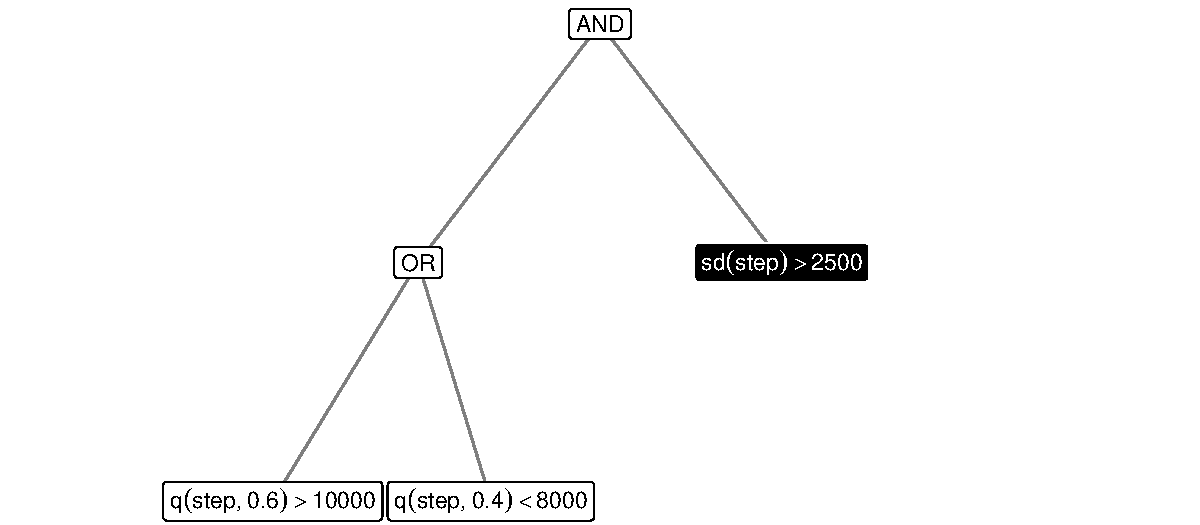
\includegraphics{index_files/figure-pdf/fig-logic-reg-1.pdf}

}

\caption{\label{fig-logic-reg}Logic regression model fitted to the three
unit tests (test1, test2, test3) and the outcome expectation (unexpect)
as the response variable. The model suggests using an OR rule to combine
test1 and test3 to predict the outcome expectation.}

\end{figure}%

\textsubscript{Source:
\href{https://huizezhang-sherry.github.io/paper-analysis-plan/index.qmd.html}{Article
Notebook}}

\textsubscript{Source:
\href{https://huizezhang-sherry.github.io/paper-analysis-plan/index.qmd.html}{Article
Notebook}}

\begin{longtable}[]{@{}
  >{\raggedright\arraybackslash}p{(\columnwidth - 10\tabcolsep) * \real{0.2424}}
  >{\raggedleft\arraybackslash}p{(\columnwidth - 10\tabcolsep) * \real{0.1515}}
  >{\raggedleft\arraybackslash}p{(\columnwidth - 10\tabcolsep) * \real{0.1061}}
  >{\raggedleft\arraybackslash}p{(\columnwidth - 10\tabcolsep) * \real{0.1970}}
  >{\raggedleft\arraybackslash}p{(\columnwidth - 10\tabcolsep) * \real{0.1364}}
  >{\raggedleft\arraybackslash}p{(\columnwidth - 10\tabcolsep) * \real{0.1667}}@{}}

\caption{\label{tbl-logic-reg}Accuracy (precision and recall) and
parsimony (independence) metrics for each individual unit test and for
the combined test rule (test1 OR test3) derived from the logic
regression model. The harmonic and arithmetic means of the three metrics
are included to evaluate the quality of the unit tests in diagnosing
unexpected step counts (more than five days with fewer than 8,000
steps).}

\tabularnewline

\toprule\noalign{}
\begin{minipage}[b]{\linewidth}\raggedright
tests
\end{minipage} & \begin{minipage}[b]{\linewidth}\raggedleft
precision
\end{minipage} & \begin{minipage}[b]{\linewidth}\raggedleft
recall
\end{minipage} & \begin{minipage}[b]{\linewidth}\raggedleft
independence
\end{minipage} & \begin{minipage}[b]{\linewidth}\raggedleft
harmonic
\end{minipage} & \begin{minipage}[b]{\linewidth}\raggedleft
arithmetic
\end{minipage} \\
\midrule\noalign{}
\endhead
\bottomrule\noalign{}
\endlastfoot
test1 & 0.48 & 0.96 & 1 & 0.73 & 0.82 \\
test2 & 0.21 & 1.00 & 1 & 0.45 & 0.74 \\
test3 & 0.59 & 0.80 & 1 & 0.76 & 0.80 \\
test1 OR test3 & 0.82 & 0.84 & 1 & 0.88 & 0.89 \\
regression tree & 0.82 & 0.84 & 1 & 0.88 & 0.89 \\

\end{longtable}

\textsubscript{Source:
\href{https://huizezhang-sherry.github.io/paper-analysis-plan/index.qmd.html}{Article
Notebook}}

\section{Applications}\label{sec-examples}

Three examples are presented to illustrate how the concept of analysis
plan can be applied to data analysis. {[}toy example{]}.
Section~\ref{sec-linear-reg} illustrates how constructing the result
universe in a linear regression model of PM10 on mortality can help
understand the impact of sample size, model specification, and variable
correlation structure on data analysis. {[}example three{]}

\subsection{Linear regression}\label{sec-linear-reg}

Consider a linear regression model to study the effect of PM10 on
mortality (provide context of using PM10 to study mortality). Analysts
may expect a significant (p-value \(\le\) 0.05) PM10 coefficient in the
linear model from the literature. This is the \emph{outcome
expectation}. There are multiple factors that can affect the outcome
expectation of linear regression, which here is called \emph{plan
expectation}, for example, 1) sample size, 2) model specification, and
3) correlation structure between variables. Adequate sample size is
required to achieve the desired power to detect the significance of PM10
on mortality. Temperature is often an important confounder to consider
in such study (add reference). From some domain knowledge, an analyst
may expect that the significance of PM10 coefficient can be attained by
adding temperature to the model. Analysts may also expect certain
correlation structure between PM10, temperature, and mortality, and the
distribution of each variable.

\begin{itemize}
\tightlist
\item
  add a paragraph to describe the simulation process
\end{itemize}

\textsubscript{Source:
\href{https://huizezhang-sherry.github.io/paper-analysis-plan/index.qmd.html}{Article
Notebook}}

\section{Discussion}\label{discussion}

\begin{itemize}
\item
  how to systematically simulate data is still unknown, sensitivity of
  the simulation to the results
\item
  plotting is a critical way to check data and they can still be frame
  into a unit test. it is a open problem to how to encode the
  visualization into the unit tests. Maybe a procedure like confirm plot
  (this looks alright to you) and then press the button to continue
\item
  currently no automated way to generate unit tests. It is interesting
  to see the automation of generating unit tests, although it requires
  the inputs from experts across a wide array of common scenarios.
\item
  There are cost and benefit on setting expectation on different
  granularity. At the lowest level, one may have a plan for each data
  entry and every data handling steps. This requires more work from the
  analysts and may not be practical in practice. For more complex
  analyses, analysts may divide the analysis into sections and set
  expectations for each. They can then focus on the specific sections
  flagged by the tests and sub-divide the sections to set expectation
  and diagnose the analysis in a hierarchical manner.
\item
  (only mention it) Software testing relies on ``oracles'' to provide
  the expected output necessary for verifying test results. For example,
  to test whether the program correctly calculates 1 + 1, one need to
  supply the correct answer, 2. However, establishing this ``correct''
  output can sometimes be challenging, where obtaining a solution may be
  difficult without the program itself. This situation leads to the
  oracle problem \citep{barr2014oracle}. In data analysis, the similar
  oracle problem can happen, as the ``truth'' of an outcome, the
  expectation, depends on the underlying theory or interpretation. For
  example, in a linear regression model, the significance of a
  coefficient may be expected or unexpected based on the theory, making
  it challenging for researcher with a different theory to assess the
  results and the analysis.
\end{itemize}

\section{Conclusion}\label{sec-conclusion}


\renewcommand\refname{References}
  \bibliography{references.bib}



\end{document}
